\newSec[HWParrot]{Parrot Drohne}{2}

Um die Problematik der COEX Drohne zu umgehen, steigt diese \Arbeit\ auf die Drohne um, welche die Idee für diese Studienarbeit ergeben hat.
Hierbei handelt es sich um die Drohne \Ar. Nachfolgend soll die Drohne und die eingebaute Sensorik näher bechrieben werden.


\newSec{Sensorik}{3}
\begin{itemize}
\item Beschleunigungssensorik
\item Magnetometer
\item Ultraschall-Abstandsmessung zum Boden
\item Frontkamera
\item Bodenkamera
\end{itemize}


\newSec[parrotROS]{Interaktion mittels \ROS}{3}

\newSec[parrotAutonomy]{Treiber \pAuto}{4}
Für die Ansteuerung der Drohne \Ar\ existiert eine Treiber, welche die Initialisierung und die Kommunukation mit der Drohne anbietet. Die \Ar\ entspricht hierbei einem Client. Der \ROS-Core wird auf dem Host-Rechner ausgeführt.
Als \ROS-seitige Schnittstelle werden verschiedene \Topic[s] und \Service[s] angeboten, welche nachfolgend näher beschrieben werden sollen.


\newSec[parrotTopics]{Topics}{4}
\begin{figure}[ht!]
\vspace{0.25cm}
\begin{center}
\fbox{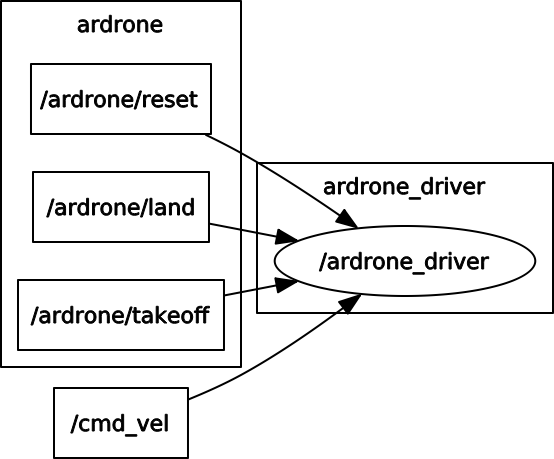
\includegraphics[width=8cm]{Pictures/RQT DroneOnly.png}}
\caption{rqt-Graph der \Ar}
\label{fig:rqtRaw}
\end{center}

\vspace{0.25cm}
Die hier gezeigten \Topic[s] beschränken sich auf die \Topic[s] zum steuern des \Quad[s] \Ar.
\end{figure}


\newSec[parrotTopicsNav]{\rTopic{NavData}}{5}
Das \rTopic{NavData} fasst alle für die verfügbaren Daten des \Quad[s] in einem Nachricht zusammen. hieraus können geeignete Informationen entnommen werden.


\newSec[parrotTopicsCMD]{\rTopic{cmd\_vel}}{5}
Entsprechend der Dokumentation werden über das \rTopic{cmd\_vel} die linearen Geschwindigkeiten und die Winkelgeschwindigkeit übertragen. Eine vorgabe der \textit{Roll-Pitch-Yaw}-Winkel ist nicht vorgesehen. \comp{parotCmdVel}\\
Entsprechen alle Attribute der \texttt{geometry\_msgs::Twist}-Nachricht dem Wert 0, schaltet die \Ar\ in einen Hover-Modus um und versucht, die aktuelle Position zu halten. Zu beachten ist, dass diese Funktion nicht für die Aufgabenstellung herangezogen werden kann, da für den studentischen Laborversuch \textit{Höhenregelung} Daten abweichend des Werts 0 über das \rTopic{cmd\_vel} übermittelt werden.


\newSec[parrotTopicsStream]{Video-Streams}{5}
Die Übertragung der Video-Daten der beiden Kameras soll an dieser Stelle lediglich erwähnt werden.


\newSec[parrotIB]{Inbetriebnahme auf separatem Rechner}{3}

Der in \refCap{parrotAutonomy} Treiber kann entsprechend folgender Anleitung isntalliert werden:\\
\href{https://ardrone-autonomy.readthedocs.io/en/latest/installation.html}{https://ardrone-autonomy.readthedocs.io/en/latest/installation.html}

Für das in dieser \Arbeit\ entwickelte Programm werden folgende \ROS-Knoten benötigt:
\begin{itemize}
\item roslaunch ardrone\_autonomy ardrone.launch
\item rosrun PosControl AutoController\\
\textit{alternativ:} rosrun PosControl ManualController
\item rosrun keyboard KeyReader
\end{itemize}


\newSec[parrotTrouble]{Troubleshooting}{3}

\newSec[parrotTroubleBattery]{Akkus}{4}
Die mit der \Ar\ zur Verfügung gestellten Akkus konnten selbst in vollständig geladenen Zustand keine zufriedenstellende Flugdauer garantieren. Hierfür wurden zwei neue Akkus von einem Dritthersteller bezogen. Die Lieferung der bestellten Akkus erfoglte in geringem zeitlichen Abstand zum Projektende.\footnote{\glqq geringer zeitlicher Abstand\grqq\ entspringt in diesem Kontext einem Zeitraum von drei Wochen. In diesem Zeitraum lag die Priorität des Autors auf der schriftlichen Ausarbeitung dieser \Arbeit.}




















